% Created 2021-09-27 Mon 11:53
% Intended LaTeX compiler: xelatex
\documentclass[letterpaper]{article}
\usepackage{graphicx}
\usepackage{grffile}
\usepackage{longtable}
\usepackage{wrapfig}
\usepackage{rotating}
\usepackage[normalem]{ulem}
\usepackage{amsmath}
\usepackage{textcomp}
\usepackage{amssymb}
\usepackage{capt-of}
\usepackage{hyperref}
\setlength{\parindent}{0pt}
\usepackage[margin=1in]{geometry}
\usepackage{fontspec}
\usepackage{svg}
\usepackage{cancel}
\usepackage{indentfirst}
\setmainfont[ItalicFont = LiberationSans-Italic, BoldFont = LiberationSans-Bold, BoldItalicFont = LiberationSans-BoldItalic]{LiberationSans}
\newfontfamily\NHLight[ItalicFont = LiberationSansNarrow-Italic, BoldFont       = LiberationSansNarrow-Bold, BoldItalicFont = LiberationSansNarrow-BoldItalic]{LiberationSansNarrow}
\newcommand\textrmlf[1]{{\NHLight#1}}
\newcommand\textitlf[1]{{\NHLight\itshape#1}}
\let\textbflf\textrm
\newcommand\textulf[1]{{\NHLight\bfseries#1}}
\newcommand\textuitlf[1]{{\NHLight\bfseries\itshape#1}}
\usepackage{fancyhdr}
\pagestyle{fancy}
\usepackage{titlesec}
\usepackage{titling}
\makeatletter
\lhead{\textbf{\@title}}
\makeatother
\rhead{\textrmlf{Compiled} \today}
\lfoot{\theauthor\ \textbullet \ \textbf{2021-2022}}
\cfoot{}
\rfoot{\textrmlf{Page} \thepage}
\renewcommand{\tableofcontents}{}
\titleformat{\section} {\Large} {\textrmlf{\thesection} {|}} {0.3em} {\textbf}
\titleformat{\subsection} {\large} {\textrmlf{\thesubsection} {|}} {0.2em} {\textbf}
\titleformat{\subsubsection} {\large} {\textrmlf{\thesubsubsection} {|}} {0.1em} {\textbf}
\setlength{\parskip}{0.45em}
\renewcommand\maketitle{}
\author{Taproot}
\date{\today}
\title{Axler 6.A exercise 9}
\hypersetup{
 pdfauthor={Taproot},
 pdftitle={Axler 6.A exercise 9},
 pdfkeywords={},
 pdfsubject={},
 pdfcreator={Emacs 28.0.50 (Org mode 9.4.4)}, 
 pdflang={English}}
\begin{document}

\tableofcontents

\section{Axler 6.A exercise 9}
\label{sec:org551390a}
\begin{quote}
Suppose \(u, v \in V\) and \(\lVert u \rVert \leq  1\) and \(\lVert v \rVert \leq  1\). Prove that
\[\begin{aligned}
  \sqrt{1-\lVert u\rVert^2}\sqrt{1-\lVert u \rVert ^2} \leq  1- | \langle u, v \rangle |
  \end{aligned}\]
\end{quote}
\section{Proof}
\label{sec:org1d97967}

\subsection{Useful Lemma}
\label{sec:org60db2a9}
\begin{quote}
\[\begin{aligned}
   \lVert u \rVert ^2 + \lVert v \rVert ^2 \geq 2 \lVert u \rVert \lVert v \rVert
   \end{aligned}\]
\end{quote}

\begin{center}
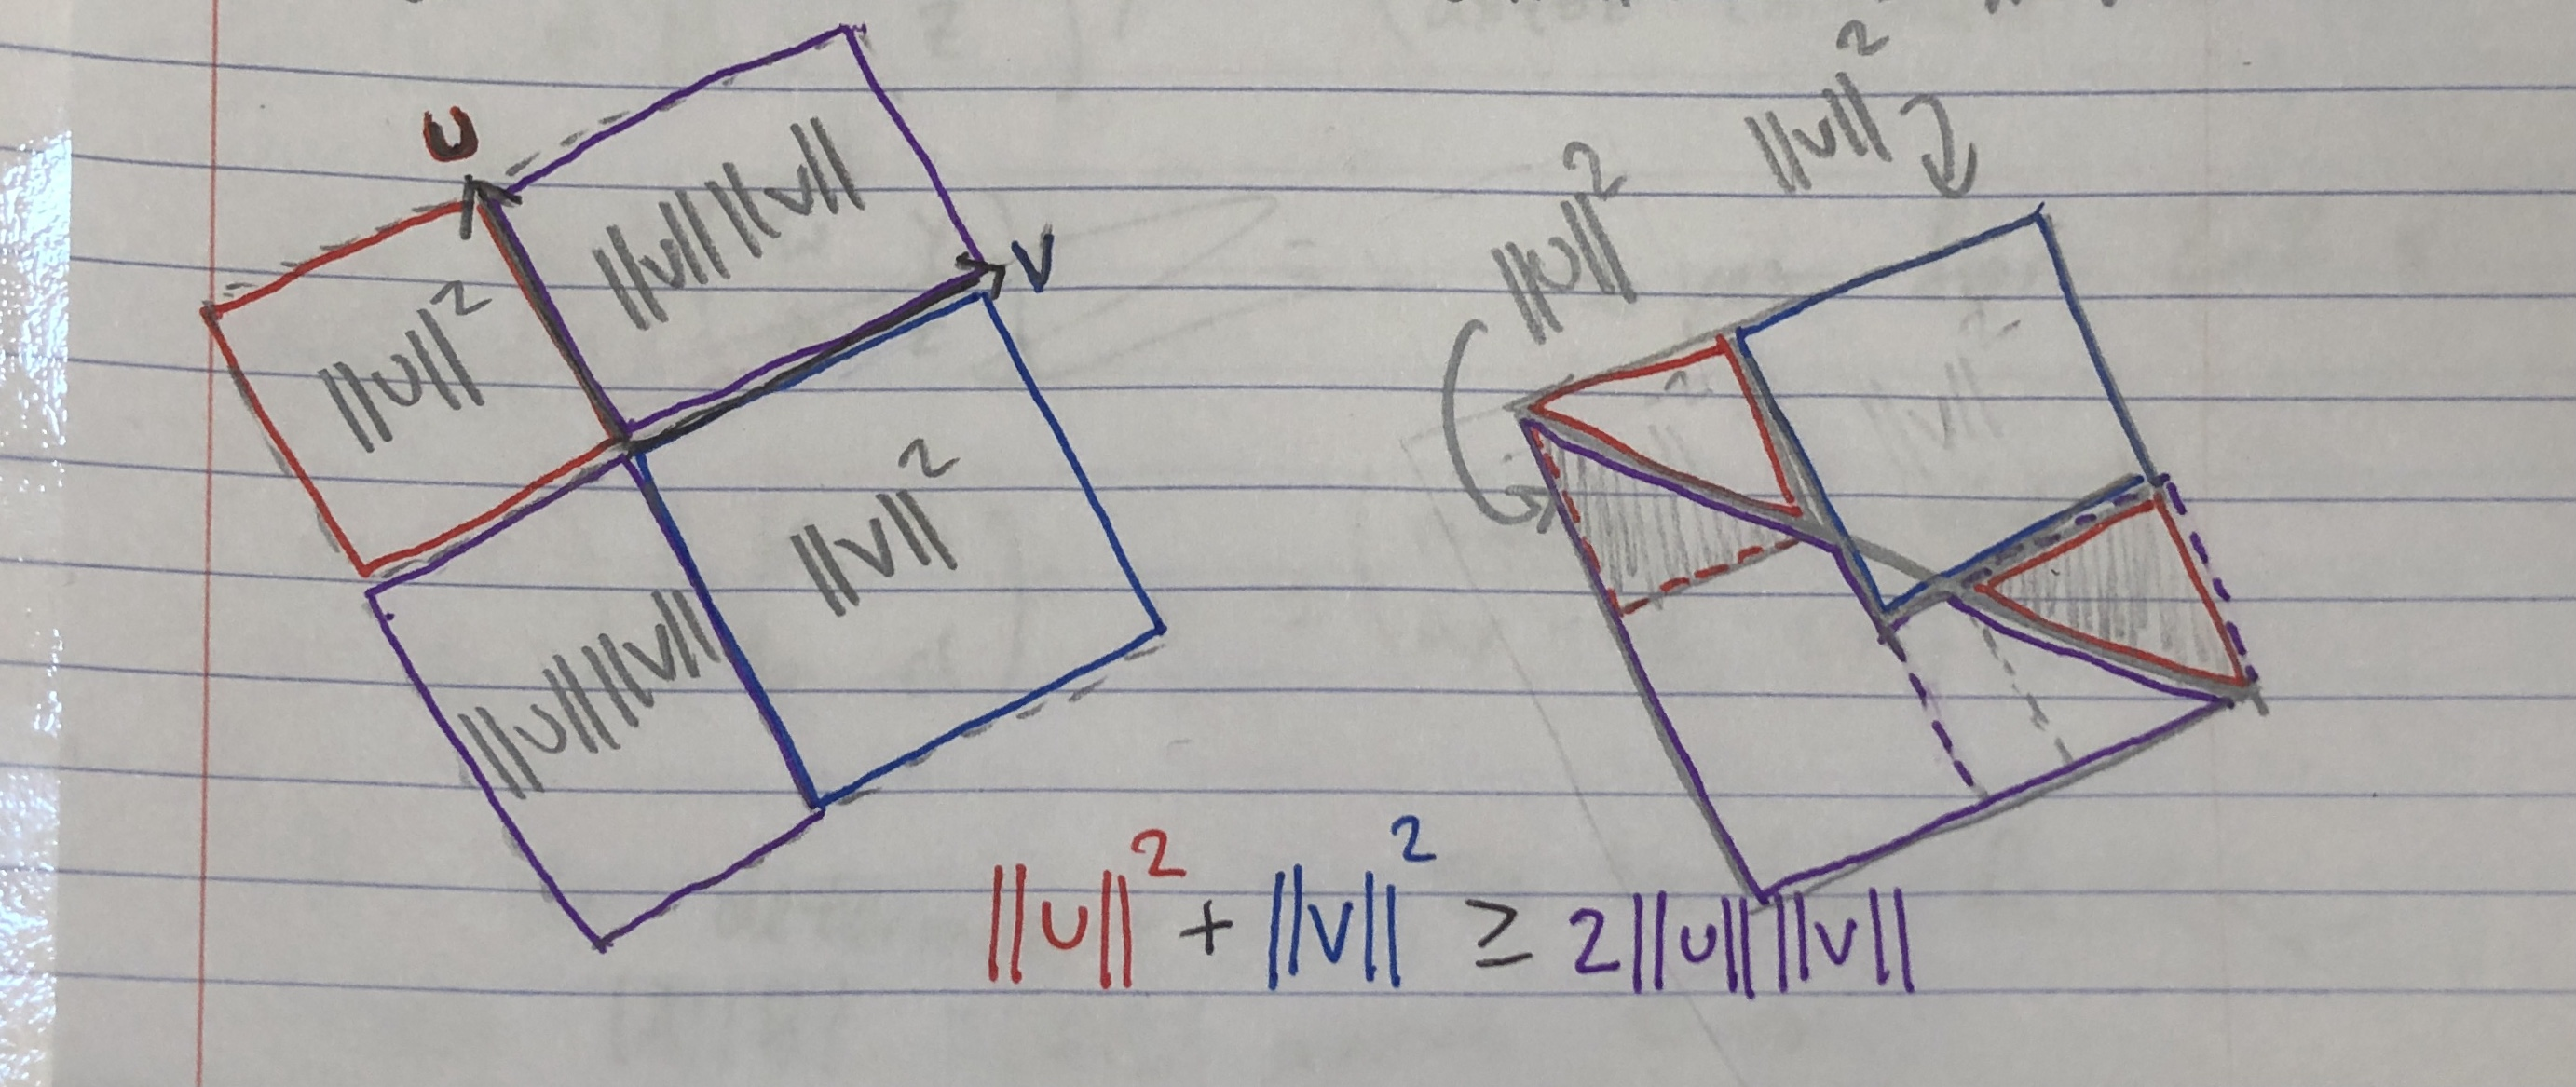
\includegraphics[width=.9\linewidth]{KBe21math530srcAxler6A9Supplement.png}
\end{center}

This proof is only valid for inner product spaces over \(\mathbb{F}^n\) and the Euclidean norm. An algebraic proof would be better.

\subsection{Cauchy-Schwarz Corollary}
\label{sec:orgbefe207}
\[\begin{aligned}
  \lvert \langle u, v \rangle \rvert &\leq \lVert u \rVert \lVert v \rVert \implies 1- \lVert u \rVert \lVert v \rVert &\leq 1- \lvert \langle u, v \rangle \rvert
  \end{aligned}\]

\subsection{Main Proof}
\label{sec:org3107106}
Now, to show that the square of the left hand side is less than or equal to the square of the right hand side,

$\backslash$[
\begin{aligned}
(1-\lVert u \rVert ^2)(1- \lVert v \rVert ^2) =& 1-\lVert u \rVert ^2 - \lVert v \rVert ^2 + \lVert u \rVert ^2 \lVert v \rVert ^2\\
=& 1- (\lVert u \rVert ^2 + \lVert v \rVert ^2 ) + \lVert u \rVert ^2 \lVert v \rVert ^2\\
\leq & 1 - 2\lVert u \rVert \lVert v \rVert + \lVert u \rVert ^2 \lVert v \rVert ^2          &&\text{by the earlier lemma}\\
=& (1-\lVert u \rVert \lVert v \rVert ) ^2\\
\leq& (1- \lvert \langle u, v \rangle \rvert ) ^2                                            &&\text{by the Cauchy-Schwarz corollary}
\end{aligned}
$\backslash$]

Taking square roots of both sides proves the desired result. \hfill \blacksquare
\end{document}
